\documentclass[UTF8]{ctexart}

\usepackage{amsmath}
\usepackage{amssymb}
\usepackage{appendix}
\usepackage{diagbox}
\usepackage{enumerate}
\usepackage{fontspec}
\usepackage{geometry}
\usepackage{graphicx}
\usepackage{subfigure}
\usepackage{url}
\usepackage{xeCJK}

\title{实现自适应空间文本分割树}
\author{王梓涵\quad 周昕逸\quad 刘权}
\date{}
\bibliographystyle{plain}

\geometry{left=2.5cm,right=2.5cm,top=2.5cm,bottom=2.5cm} 
\pagestyle{plain}

\begin{document}
\maketitle

\linespread{0.5}
\setlength{\parskip}{0.5\baselineskip}

\section{理论介绍}

在日常的信息传播中,常常需要处理用户所提供的一系列包含空间和关键词的查询项。例如:一些基于位置信息的推荐系统可根据用户的需求推送相关产品的信息,Twitter等社交网络可分析用户发布的内容及附带的地理位置标签推送他们感兴趣的内容。本文实现的自适应空间文本分割树(Adaptive spatial-textual Partition Tree,以下简称AP树)可以通过自动计算关键词和空间因子两种分割方式的代价选择合适的匹配方式。

AP树的实现有三大挑战。第一,在实际应用中的数据量极大,算法效率的提升可以节省很多成本。第二,算法吞吐量要大以应对源源不断的包含空间文本信息的对象流。第三,需要建立新的空间因子和关键词的索引机制用于不同的分配方法。

AP树的基本运算包含三个部分。匹配对象和查询项的算法,计算关键词和空间因子分割代价的模型和建立索引的算法。

AP树包含三种类型的结点:关键词结点(k-node),空间结点(s-node)和查询项结点(q-node)。一棵AP树的叶子结点都是q-node,每一个查询项都可根据其关键词和空间因子被分配入一个或多个叶子结点中。运用关键词分割方法的结点称为k-node。我们认为所有的关键词都包含于一个有序的词典中,它们的相对位置是确定的,因此可以比较大小。每一层的k-node中包含了其叶子结点对应的查询项的第结点层次个关键词的划分(cuts)。运用空间面积分割方法的结点称为s-node。每一层的s-node中包含了其叶子结点对应的查询项的面积划分(cells)。如果一个查询项没有足够的关键词,无法寻找到一个对应的cut,就用一个dummy cut保存;如果一个查询项的覆盖面积已经包含一个s-node的覆盖面积,就用一个dummy cell保存。

在匹配对象时,使用深度优先搜索法。如果当前结点是q-node,则判断该对象是否与q-node中的查询项匹配,如果匹配则可等待输出。如果当前结点是s-node,则访问它的cell和dummy cell。如果当前结点是k-node,则访问它的cut和dummy cut。

AP树还提供了一个计算两种分割匹配算法的代价的模型。匹配代价$C(P)$的定义为:\[C(P)=\sum_{i=1}^f \mathbf{w}(B_i)\times \mathbf{p}(B_i)\]其中$B$是一种分割方式,$\mathbf{w}(B)$是与$B$有关的查询项的个数,$\mathbf{p}(B)$是$B$的击中概率,即在对象匹配过程中$B$被访问的可能性。在关键词分割法中,$\mathbf{p}(B)=\sum_{w\in B} \mathbf{p}(w)$,其中$\mathbf{p}(w)=\frac{freq(w)}{\sum_{w\in P}freq(w)}$,$freq(w)$为关键词$w$在所有查询项中出现的频率。在空间分割法中$\mathbf{p}(B)=\frac{Area(B)}{Area(N)}$,$Area(B)$是$B$的面积,$Area(N)$是结点$N$的区域面积。接着使用启发式算法寻找使得匹配代价最小的关键词的分割和空间的分割。

AP树还提供了建立索引的方法。使用两个标志$kP$和$sP$来表示所有的查询项是否可以进一步地进行关键词的分割和空间的分割,并通过计算两种分割方式的代价$C_k$和$C_s$确定当前结点使用哪种分割方式。


\section{代码实现}

\subsection{接口设计}
首先定义所涉及的两个结构体:空间文本对象\texttt{STObject}以及查询项\texttt{Query}。\texttt{STObject}有两个成员:\texttt{Pointf}类型的位置\texttt{location}以及\texttt{std::set<std::string>}类型的关键词集合\texttt{keywords}。\texttt{STObject}也有两个成员:\texttt{Boundf}类型的方形区域\texttt{region}和\texttt{std::set<std::string>}类型的关键词集合\texttt{keywords},其中\texttt{Boundf}为由两个\texttt{Pointf}确定的轴对齐包围区域。类的使用者需要通过这两个结构来和类进行交互。

本文所实现的AP树,是一种空间文本分割树,定义抽象的空间文本分割树类\texttt{STTree},其有一个纯虚函数\texttt{std::vector<Query> Match(const STObject \&) const}。用户通过输入\texttt{STObject},可获得查询项,存放于一个\texttt{std::vector}中。AP树类\texttt{APTree}继承自\texttt{STTree}。\texttt{APTree}的构造函数声明为\texttt{APTree(const std::vector<std::string> \&vocab, const std::vector<Query> \&queries, size\_t nCuts, size\_t threshold)},其中\texttt{vocab}为所有的关键词,\texttt{queries}为需要注册的查询项,\texttt{nCuts}即论文中的$f$,为每个k-node或s-node的建议分割数目,\texttt{threshold}即论文中的$\theta_q$,为每个q-node的最大查询项容量。

\subsection{存储实现}
由于AP树存储的数据体量大,树的构建和查询算法较为复杂,为了能够发挥AP树的优势,在内部存储方式的实现上需要一定的构思。

首先介绍AP树内部对于空间文本对象和查询项的存储。在\texttt{APTree}内部,使用\texttt{STObjectNested}和\texttt{QueryNested}来分别表示这两种结构。在两种结构中,位置信息,即\texttt{location}和\texttt{region}保持原样,而\texttt{keywords}变为\texttt{std::vector<size\_t>}类型,其中\texttt{std::vector}所存储的是该关键词在关键词词汇\texttt{vocab}中的索引。考虑到字符串的比较较为耗时,而整数的比较效率较高,在建树和查找的过程中可以直接对序号进行操作,而非对字符串。同时,由于AP树算法中有对\texttt{keywords}随机访问的需求,应该将其从原来的\texttt{std::set}转为\texttt{std::vector}以实现高效的随机访问。

然后介绍关键词分割方案和空间分割方案的存储表示。关键词分割方案用\texttt{KeywordPartition}结构体表示,其成员包括:类型为\texttt{std::vector<KeywordCut>}的分割序列\texttt{cuts},其中\texttt{KeywordCut}为关键词序号的闭区间;类型为\texttt{std::map<KeywordCut, std::vector<QueryNested *>>}的查询项查找表\texttt{queries},用来表示每个关键词闭区间对应哪些查询项,注意到这里使用的是\texttt{QueryNested}的指针类型,这是为了节约运行时内存占用,避免\texttt{QueryNested}的多次复制;类型为\texttt{std::vector<QueryNested *>}的dummy cut表\texttt{dummy};还有一个表示该分割方案代价的浮点数\texttt{cost}。空间分割方案用\texttt{SpatialPartition}结构体表示,其成员包括:类型为\texttt{size\_t},在X、Y轴上个各自的分割数目\texttt{nPartX}、\texttt{nPartY};类型为\texttt{std::vector<double>}的分割位置\texttt{partX},\texttt{partY},注意这两个\texttt{std::vector}的\texttt{size()}各自比\texttt{nPartX},\texttt{nPartY}多一个,为了代码清晰,不使用它们的\texttt{size()}信息;类型为\texttt{std::unique\_ptr <std::vector<QueryNested *>>}的单元格查询项序列\texttt{cells},注意这是一个一维的数组,一个二维的单元格索引需要通过运算转为一维的数组索引;剩下的\texttt{dummy}和\texttt{cost}与\texttt{KeywordPartition}相同,不作赘述。

最后介绍AP树的结点类型\texttt{Node},由于AP树有三种结点类型,而每个结点的子节点的类型父节点是不清楚的,这里使用一个\texttt{NodeType}枚举来标记每个子节点的类型;同时每个结点需要存储结点的区域\texttt{bound}。对于三种结点各自的信息,定义了\texttt{Node}的内部结构体来储存。为了节约结点空间,使用\texttt{std::unique\_ptr}来实现较为灵活的管理,默认状况下为\texttt{nullptr},当结点信息完备时,再根据结点类型动态地分配相应的存储空间。q-node类型\texttt{Node::QueryNode}内只需要存储一个\texttt{std::vector<QueryNested>}即可;k-node类型\texttt{Node::KeywordNode}和s-node类型\texttt{Node::SpatialNode}的成员分别与\texttt{KeywordPartition}和\texttt{SpatialPartition}成员类似,不同之处在于\texttt{Node::KeywordNode}和\texttt{Node::SpatialNode}内不需要存储\texttt{cost}信息,且各自的查找表内存储的是\texttt{std::unique\_ptr<Node>}的数组,而非\texttt{QueryNested *};由于k-node和s-node内共有dummy cut,考虑将其放在\texttt{Node}的一个\texttt{std::unique\_ptr}中,避免重复定义。这样一来,\texttt{APTree}析构的时候所有内存空间可以自动回收,不需要手动\texttt{delete},也不会造成内存泄漏。

\subsection{运算实现}
AP树的相关算法基本根据原论文所给的伪代码来实现,以下的介绍只作大致思路的梳理和部分要点的提示。

在构造函数里,首先根据参数\texttt{vocab}将\texttt{Query}转成\texttt{QueryNested},并取址,建立\texttt{std::vector <QueryNode *>},然后从根节点开始调用私有\texttt{build}函数。在\texttt{build}函数内,若当前结点判定为q-node,则将传入的\texttt{std::vector<QueryNode *>}内的指针全部取值储存在\texttt{Node::QueryNode}中;不然则调用私有的\texttt{keywordHeuristic}和\texttt{spatialHeuristic}尝试关键词和空间分割,取代价小的分割方式确定节点类型,将相关信息赋予结点,继续下一层递归。要注意,\texttt{Node}的内存空间要在主调用的\texttt{build}函数内分配,其成员的数据在被调用的\texttt{build}函数内赋给。

下面介绍一下\texttt{keywordHeuristic}和\texttt{spatialHeuristic}内的实现。由于它们均为启发式算法,有相似的思路。首先,对传入的查询项进行\textbf{统计},关键词分割时分别统计当前offset以及所有offset的词频,空间分割时统计边界位置。然后,对统计的对象进行\textbf{均分},关键词分割时均分关键词到每个cut,空间分割时均分边界到每个cell。接着尝试改变划分的边界,找到局部最优的划分,\textbf{改善}整体的代价。最后,利用找到的最佳划分,将查询项\textbf{分配}到每个cut或者cell内,算法结束。

在\texttt{Match}函数内,首先将\texttt{STObject}转成\texttt{STObjectNested},调用私有的\texttt{match}函数进行匹配,匹配算法完全按照论文中的伪代码实现。将得到的\texttt{std::set}内的\texttt{QueryNested}转成\texttt{Query},返回给类的使用者。

最后介绍三个和容器中有序元素相关的工具函数:\texttt{commonElements}能够寻找两个容器中的相同的元素,对于大小为$m$和$n$的两个容器,以$O(m+n)$的时间复杂度找到相同元素,主要用于\texttt{spatialHeuristic}中寻找两个坐标轴上特定范围内的查询项的交集。\texttt{isSubset}能够判断一个容器中的元素组成的集合是否是另一个容器中元素集合的子集,同样可以达到$O(m+n)$的时间复杂度,主要用于验证\texttt{QueryNested}和\texttt{STObjectNested}关键词之间的包含关系。\texttt{rangeSearch}用查询某个类型为\texttt{Type}的值,在一个用有序数组\texttt{std::vector<Type>}表示的若干首尾相接区间左端点中的索引。该算法类似二分查找,不过验证的是区间和值的包含关系,而非值的相等关系,主要用在查找某个点在q-node中所对应的cell的二维索引。\texttt{Node::KeywordNode}中的\texttt{Search}成员函数和\texttt{rangeSearch}行为类似,不过其针对的区间\texttt{KeywordCut}不保证首尾相接。

\section{性能测试}


\section{评价}
\subsection{优势}
原论文中也提了几种其他用于解决类似问题的结构,如$\mathrm{R^t}$树和IQ树。它们有一个共通点:无论查询项中关键词和空间信息有何特点,在建立索引时空间因素始终优先于关键词因素。相比而言,AP树有以下几点优势:
\begin{enumerate}
    \item AP树在处理不同的数据集时匹配对象的速度快。因为对有些数据集来说关键词和空间两种匹配模式的效率差别很大,AP树可以很好地利用它的自适应性选择最优的匹配算法。
    \item 当AP树应对较多查询项时,依然能保证较高的效率。
    \item AP树可以自动维护它的结构。当工作量发生变化时,它可以根据阈值重构自己的结点,体现出它的自适应性。
\end{enumerate}

\subsection{不足}
\begin{enumerate}
    \item AP树对于空间的需求量较大。在存储实现中可以看到,尽管对于结点的存储方案已经做了一定优化,但是单个结点占用空间依然较大。在树的构建过程中,每一层递归都需要储存对应结点查询项的统计信息。当查询项的总数较大时,势必造成内存占用的激增。在我们的测试中,在注册了5000个查询项后,内存占用就超过了90MB。如果是实际应用中上百万的查询项,其内存占用是相当巨大的。
    \item AP树的构造较为复杂。AP树由于要对两种分割模式进行混合,要实现它就必须要比其它单模式的分割树付出多一倍以上的工作量。本项目关于\texttt{APTree}的实现代码,仅仅实现了AP树最基础的功能,还不包括查询项的维护,就已有六百余行。如果要将它整合到一个可实际应用的数据库系统中的话,其工作量是可想而知的,这显然不利于一个数据库系统的维护、更新和迭代。
\end{enumerate}

\section{未来工作}
由于时间和开发者能力所限,该项目还有许多不完善的地方,在将来可能会对以下方面进行改进或补充。
\begin{enumerate}
    \item 当前的\texttt{APTree}中所有的查询项只能在构造函数里一次性注册,而原论文中作者提到可以利用KL散度的计算对查询项进行动态地注册和注销。由于作者并未详细描述其算法,且此项目开发者尚不具备信息论的相应知识,所以并未实现。今后可以尝试阅读相关的文献,在\texttt{APTree}中增加\texttt{Register}和\texttt{Unregister}成员方法,实现该功能。
    \item 我们的实验中只实现了AP树一种结构,并未实现论文中提到的其他空间文本分割结构,所以无法进行比较,不能体现AP树的优势。今后考虑实现IQ树、$\mathrm{R^t}$树、顺序关键词字典树等结构,进行横向比较。
    \item 我们当前的测试只考察了\texttt{APTree}的执行时间,分析了时间复杂度方面的性质,对于其内存占用的情况只做了定性的分析与简单的记录。今后考虑直接使用或设计相应的测试工具,对其内存的使用情况进行具体的跟踪。
\end{enumerate}

\newpage

\begin{appendices}

\section{源代码}
本文所实现的AP树源代码仓库在GitHub上进行托管:\url{https://github.com/wzh99/AP-Tree},采用MIT许可证。

\section{数据集来源}
本文测试所使用的关键词数据集来自US Board on Geographic Names(\url{http://geonames.usgs.gov})

\begin{figure}[htbp]
    \centering
    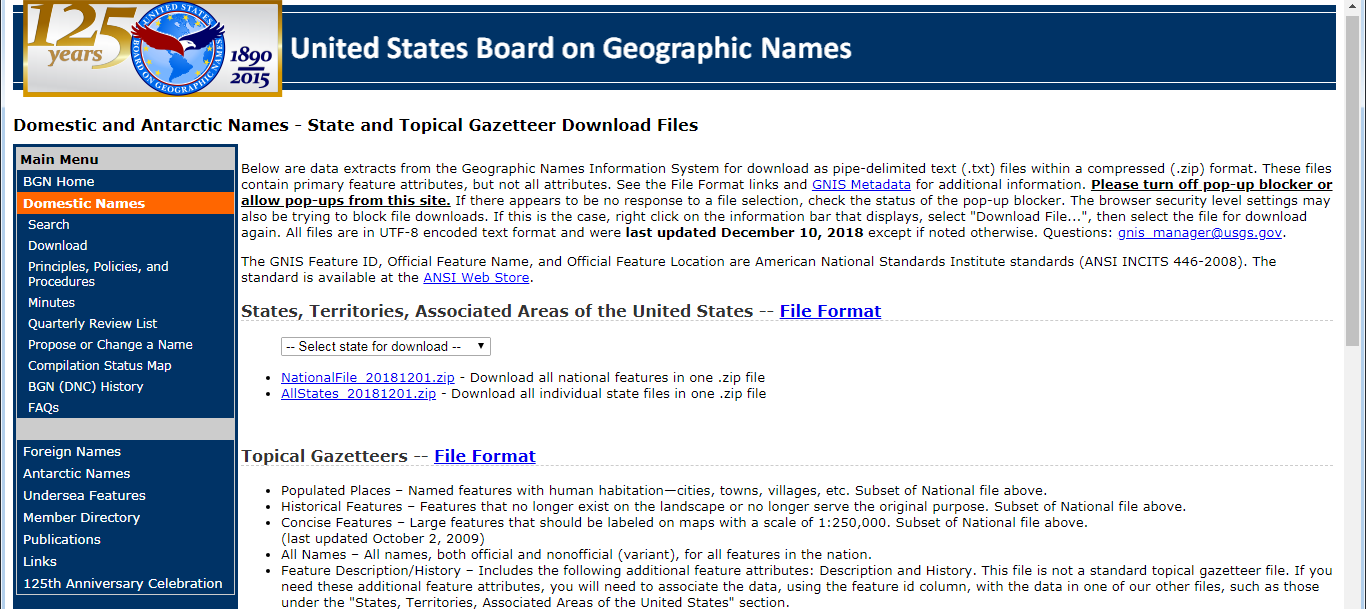
\includegraphics[width=\textwidth]{gn.png}
    \caption{US Board on Geographic Names网站}
\end{figure}

\section{分工}
\begin{itemize}
    \item \textbf{代码实现:} 王梓涵
    \item \textbf{数据测试:} 刘权
    \item \textbf{报告撰写:} 周昕逸\quad 王梓涵\quad 刘权
\end{itemize}

\end{appendices}

\end{document}